\documentclass[10pt]{article}
\usepackage{amssymb,amsmath,amsfonts,graphicx,color, cite}
\usepackage[justification=centering]{caption}
\newcommand{\bbR}{{\mathbb R}}
\newcommand{\bbZ}{{\mathbb Z}}
\newcommand{\bbS}{{\mathcal S}}
\newcommand{\bbK}{{\mathcal K}}
\newcommand{\bbV}{{\mathcal V}}
\newcommand{\bbI}{{\mathcal I}}
\newcommand{\bbC}{{\mathcal C}}
\newcommand{\bbL}{{\mathcal L}}
\newcommand{\remove}[1]{}

\newtheorem{observation}{Observation}
\newtheorem{fact}{\noindent {\bf Fact}}

\begin{document}
\section{Outlier detection scheme} We now use the weighted projection quantiles for the purpose of detecting multivariate outliers. Relative to a multivariate data cloud, multiple outliers can either lie far away from majority of the data in a separate small cluster of points, or they may be scattered without any noticeable clumping. While there do exist $k$-nearest neighbor based \cite{lof} or depth-based \cite{dang10, chen09} outlier detection methods, they only concentrate on local or global properties of a dataset, respectively. Here we combine our idea of depth outlined in section ? with a $k$-nearest neighbor distance measure to devise an outlier score for each observation in a multivariate dataset that can detect clustered or scattered outliers based on different values of a tuning parameter.

\paragraph{Definition}Consider iid observations ${\bf X} = \{{\bf X_1},...,{\bf X_n}\} \in \mathbb{R}^{n\times p}$ from a multivariate distribution $F$. For any point ${\bf x} \in \mathbb{R}^p$ suppose $\bar d_k({\bf x},{\bf X})$ and $D({\bf x}, {\bf X})$ are its $k$-nearest neighbor distance and WPQ-depth based on the data, respectively. The the depth-based outlier score for $x$ is defined as:

$$ O_{D,\alpha}({\bf x}; {\bf X}) = \alpha. \log (\bar d_k({\bf x},{\bf X})) - (1 - \alpha)\log (D({\bf x}, {\bf X}))$$
where $\alpha \in [0,1]$ is the tuning parameter.

\paragraph{}For $\alpha=0$ this score becomes the negative log of the depth function, while $\alpha=1$ makes this same as the log of mean kNN distance. This outlier score is defined based on the reasoning that a point far isolated from the rest of the data will always have a low depth, but whether it has a high kNN distance or not depends  on if it is part of a small isolated clump of points or a single isolated point. For small values of $\alpha$, $O_{D, \alpha}$ puts more emphasis on isolated points. On the other hand, for $\alpha$ close to 1 high values of the outlier score will tend to identify low-depth isolated points.

\subsection{Simulations}We now consider two simulation scenarios to demonestrate the performance of our outlier score at different values of $\alpha$. The $k$ to obtain mean kNN distance is fixed at $\lfloor \sqrt{n} \rfloor$, and the value of tuning parameter to compute kernel-based sample weights is set at 0.2.

\paragraph{}In the first setup we consider a 500-size sample, 95\% of which are from $\mathcal{N}((0,0)',I_2)$ and the other 5\% drawn from $\mathcal{N}((10,10)',I_2)$. The second setup also contains 500 data points, the last 25 having each element of their mean vector drawn from $\{\pm 6, ..., \pm 10\}$. Since the first group has clustered outliers, a smaller value of $\alpha$ should be able to identify points in the outlying cluster, while in the second setup a higher $\alpha$ should result in high score for points with a large mean nearest-neighbor distance and small depth, i.e. the scattered outlier points. Rows 2 to 4 in Fig. 1 give the index plots for outlier scores for these two scenarios, computed considering $\alpha = 0.05, 0.5, 0.95$. Points 1 to 475 are colored green and the last 25, which are situated away from the main data cloud, are colored red. For the first group of samples, $\alpha = 0.05$ and 0.5 give a better distinction between the two populations, while in the second group this is best achieved for $\alpha=0.5$ and 0.95.

\begin{figure}[h]
	\centering
		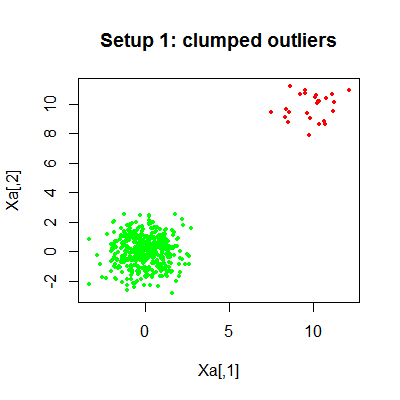
\includegraphics[height=4cm]{outlier_sim11.png}
		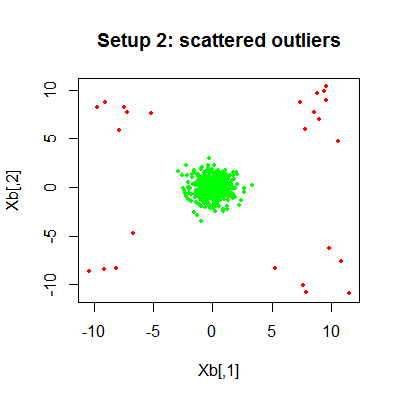
\includegraphics[height=4cm]{outlier_sim21.png}\\
		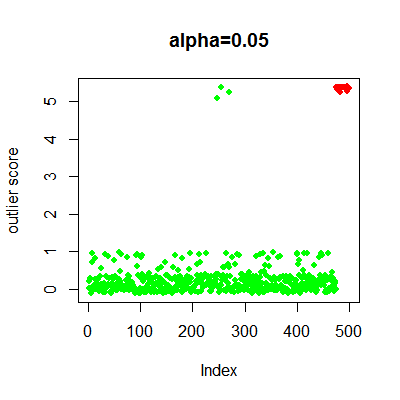
\includegraphics[height=4cm]{outlier_sim12.png}
		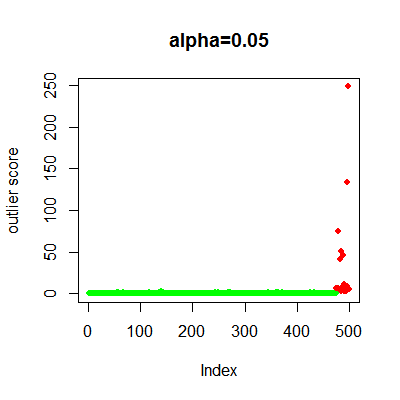
\includegraphics[height=4cm]{outlier_sim22.png}\\
		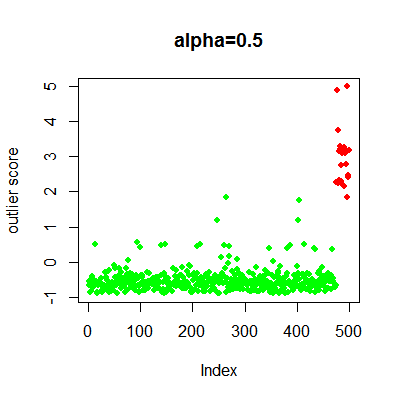
\includegraphics[height=4cm]{outlier_sim13.png}
		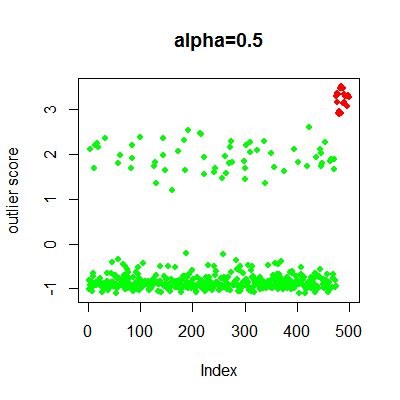
\includegraphics[height=4cm]{outlier_sim23.png}\\
		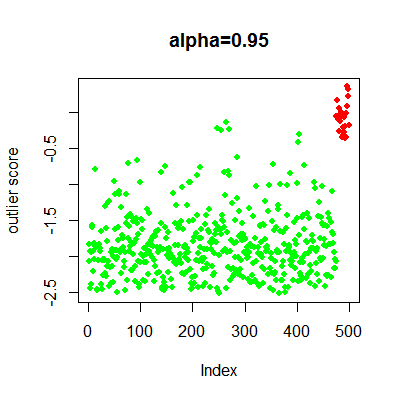
\includegraphics[height=4cm]{outlier_sim14.png}
		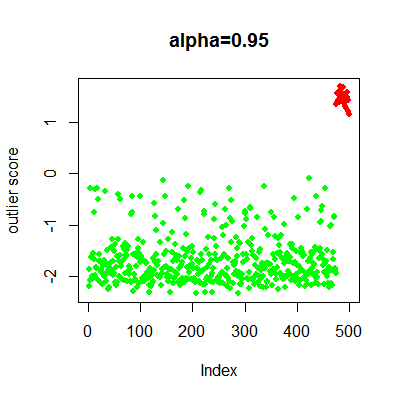
\includegraphics[height=4cm]{outlier_sim24.png}\\
	\label{fig:fig2}
	\caption{Scatter plot (top row) nd index plots (rows 2-4) for simulation setup 1 (left) and 2 (right)) $\alpha = 0.05, 0.5, 0.95$}
\end{figure}

\subsection{Real data examples}

\begin{figure}[t]
	\centering
		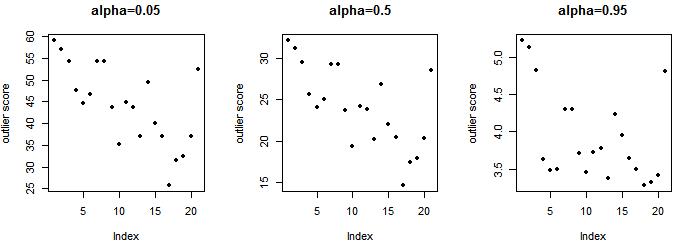
\includegraphics[height=4cm]{outlier_stackloss.png}\\
	\label{fig:fig4}
	\caption{Outlier scores for stackloss data}
\end{figure}

\begin{figure}[t]
	\centering
		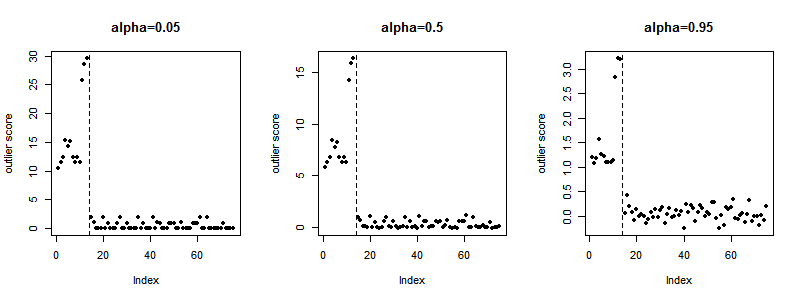
\includegraphics[height=4cm]{outlier_hbk.png}\\
	\label{fig:fig5}
	\caption{Outlier scores for Hawkins-Bradu-Kass data \\(Dotted line at index = 14)}
\end{figure}

\paragraph{Stackloss data}This dataset due to Brownlee \cite{stackloss} has 21 observations from a plant regarding oxidation of Ammonia to Nitric Acid, and has 3 predictors: air flow, cooling temperature and concentration of acid; and percentage of ingoing Ammonia that escapes the oxidation process as response variable.The stackloss dataset has been widely used for detecting outliers in regression or unsupervised analysis. For example, the analysis of only the predictor variables due to Hadi \cite{hadi92} identifies observations \{1,2,3,21\} as potential outliers, while the bayesian model averaging-based approach taken by Hoeting \textit{et al}\cite{hoeting96} identifies observations 1, 3, 4 and 21 as outliers.

\paragraph{}We set aside the response variable and calculate outlier scores based on the 3 predictors. Fig. 3 shows the scores for $\alpha = 0.05, 0.5$ and 0.95. For the first two plots, \{1,2,3\} are the top few point with high outlier scores. For $\alpha = 0.95$, there is considerable difference of scores between \{1,2,3,17,21\} and other points.

\paragraph{Hawkins, Bradu amd Kass data}This artificial dataset given by Hawkins \textit{et al} \cite{hbk} consists of 75 observations and 4 variables (3 predictors and 1 response variable). The first 10 observations are high influential points while observations 11 to 14 are good leverage points. Analysis using classical methods like Mahalanobis' distance or Cook's distance only correctly identifies 11-14 as outliers and masks points 1 to 10. Hadi's unsupervised method of robust outlier detection \cite{hadi92} correctly identifies all 14 points as outliers. Our analysis of the 3 predictor variables using depth-based outlier scores (Figure 4) replicates Hadi's finding. The choice of the tuning parameter does not seem to matter here, although a better distinction is achieved at lower values of $\alpha$, i.e. higher proportion of the depth part in outlier score.

\subsection{Analysis of DNA alteration data}We now attempt to apply the outlier detection scheme to improve performance of certain classification methods.

\bibliographystyle{plain}
\bibliography{outlierbib}

%\begin{figure}[t]
%	\centering
%		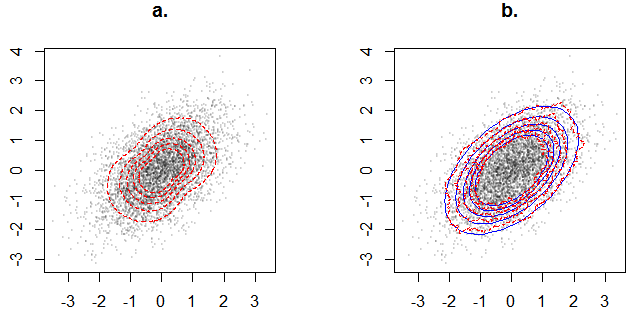
\includegraphics[height=5cm]{Sim_bvn.png}\\
%		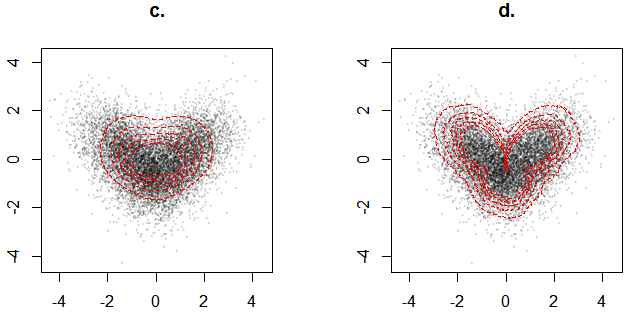
\includegraphics[height=5cm]{Sim_mixsym.png}\\
%		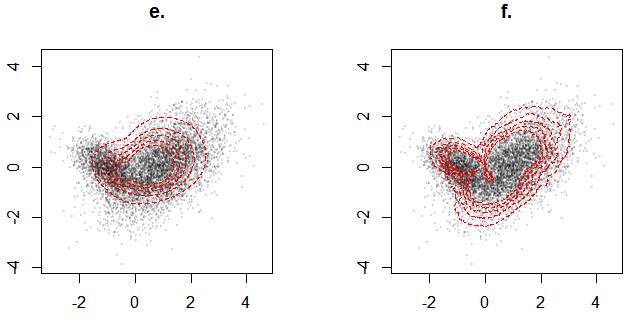
\includegraphics[height=5cm]{Sim_mixasym.png}\\
%		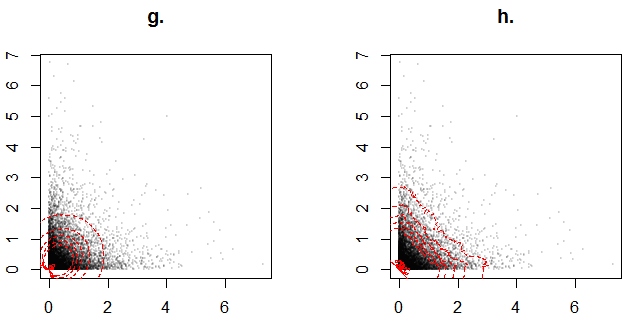
\includegraphics[height=5cm]{Sim_exp2.png}
%	\label{fig:fig1}
%	\caption{(Left) PQ and (Right) WPQ profiles for the four simulation scenarios. Blue lines in panel b represent actual confidence ellipsoids}
%\end{figure}
\end{document}